\section{Conceptual diagrams as digital documents}
\label{appendixB}

The treatment of conceptual diagrams as form of data is not obvious, so it
shall be justified in the following. Figure~\ref{fig:moody2009fig6} is used by
\textcite{Moody2009} to illustrate a specialization of the theory of
communication by \textcite{Shannon1948} to the domain of visual notations:
diagrammatic communication consists of two complementary processes: encoding
and decoding. A diagram (signal) is decoded and encoded using a visual
notation, which defines a set of conventions that both sender and receiver
understand. The diagram can vary by noise, that are minor differences in sizes,
colors, positions etc.  \hspace{5mm}

\begin{figure}[b]
\centering
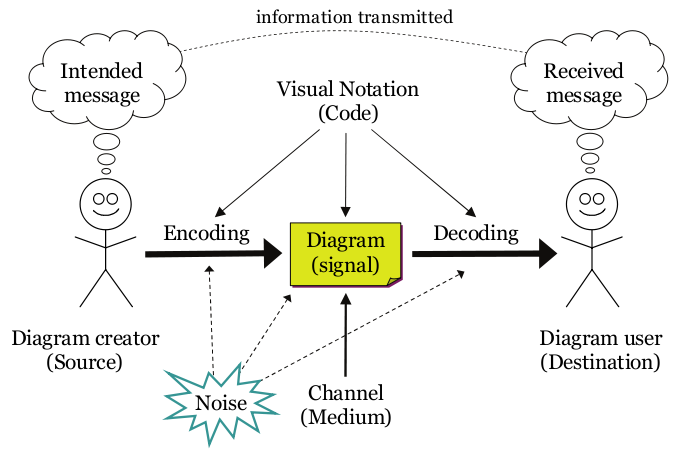
\includegraphics[width=0.7\linewidth]{img/moody2009fig6.png}
\caption{Theory of Diagrammatic Communication as by \textcite{Moody2009}}
\label{fig:moody2009fig6}
\end{figure}

Moody defines the medium (channel) as ``the physical form in which the diagram
is presented (e.g., paper, whiteboard, and computer screen)''. To digitize the
diagram from physical form to digital data, we must identify and encode its
visual symbols and the rules how symbols are combined (see
section~\ref{sec:diagramproperties}). The possibility of such encoding can be
shown by mapping the diagram to another notation, such used in
figure~\ref{fig:moodyvariant}.

\begin{figure}
\centering
\begin{tikzpicture}[
	split/.style={rectangle split, rectangle split parts=2,draw},
	shape2/.style={regular polygon,regular polygon sides=5,draw,minimum width=10mm},
	shape3/.style={ellipse,draw,text width=15mm}]

\node[split,line width=2pt] (signal) {Diagram\nodepart{two}signal};

\node[shape2,left=30mm of signal] (s) {~};
\node[shape2,right=30mm of signal] (d) {~};

\node[split,below=0 of s] (source) {Diagram creator\nodepart{two}Source};
\node[split,below=0 of d] (destination) {Diagram user\nodepart{two}Destination};

\node[shape3,above=0 of s] (im) {Intended message};
\node[shape3,above=0 of d] (rm) {Received message};

\draw[dashed,->] (s) to node[fill=white,name=enc] {Encoding} (signal);
\draw[dashed,->] (signal) to node[fill=white,name=dec] {Decoding} (d);

\draw[out=60,in=120,line width=2pt] (im) to node[fill=white] {information transmitted} (rm);

\node[split,above=8mm of signal] (notation) {Visual Notation\nodepart{two}Code};
\draw[dotted,->] (notation) -> (signal);
\draw[dotted,->] (notation) -> (enc);
\draw[dotted,->] (notation) -> (dec);

\node[split,below=15mm of signal] (channel) {Channel\nodepart{two}Medium};
\draw[ultra thick,->] (channel) -> (signal);

\node[shape=circle,draw,left=4mm of channel] (noise) {noise};
\draw[->] (noise) -> (enc);
\draw[->] (noise) -> (signal);
\draw[->] (noise) -> (dec);

\end{tikzpicture}
\caption{Figure~\ref{fig:moody2009fig6} in different layout}
\label{fig:moodyvariant}
\end{figure}

The readability differs between both diagrams, but they are formally equal, in
the same way as text in different typefaces, size, and layout can be equal if
encoded in \term{Unicode} (see example~\ref{ex:loremipsum}).  Although there is
no Unicode standard for conceptual diagrams, an encoding is possible given a
set of possible visual symbols and combination rules. For this reason
conceptual diagrams can be analyzed as data just like text in Unicode or any
other \term{writing system}.

